\chapter{Smart Contract and Distributed Ledger Technology}

\section{Ledger}
Ledger is a principal book or computer file for recording transactions measured in terms of unit account with specific balance for each account\cite{Markos}.

\subsection{Distributed Vs. Undistributed }
the difference between decentralized and distributed is made by Baran(1964). decentralized means there is no single point to make a decision. It contains central hierarchy nodes. Each node makes up a decision for own self and the system gathers all responses as resulting behavior. In a distributed system, the process spread across all nodes and there are no central nodes. The main difference is that a decentralized database is the collection of independent databases, while distributed is the single database that is spread multiple inter-connected computers in different locations. \textit{Ozsu and Valduriez} define a distributed database as a "collection of multiple, logically interrelated databases distributed over a computer network and distributed database makes a transparent distribution to all users"\cite{Ozsu}. Based on this definition Blockchain technology adheres to both definitions, as it appears as a single system to its users and performs a task in a network. Thus, Blockchain is a form of a distributed computing system.\cite{Markos}.


\section{Distributed Ledger Technology(DLT)}
DLT is the method of keeping a distributed ledger on networks of a computer. DLT uses a consensus technique for adding a new node(participant) over the network. Similarly, This is the digital record that shared across participant and the records held by each node or participant. The term 'blockchain' is the most well-known type of DLT and are used by many best-known instances of DLT.\\
A distributed ledger can be either permissionless or with permission, regarding be private or public. 
Most of the distributed ledger is permissionless and public means anyone can easily join to network and see all entries. But in financial fields, distributed ledgers are restricted to members of each participant and they are 'private' networks. Furthermore, in financial fields exist also commercial sensitivity about the privacy of data related to each participant. In another word, no one wants that data to be seen by the other participant. therefore, participants can see their data and transaction on the network.\\
Recently, blockchain as a type of distributed ledger become the most popular and widely used in diverse fields.  one of the outstanding usages of blockchain is Ethereum which extends initial bitcoin blockchain with features such as smart contracts that enable to distribute of data on the blockchain securely.
Also, there is an increasing demand to integrate data stored in distributed ledger with other external sources. And also integrate smart contracts with the service available on the web. This is where linked data comes to play to provide sufficient access to data and smart contracts also stored on Ehereum blockchain via semantic web technology stack\cite{Third}.

\section{Blockchain}
Blockchains are the distributed records for digital events and they are structured as a chain of linked data stored in individual database or computer over network\cite{Third}.
Blockchain is organized into blocks. Each block is identified by cryptography hash that refers to a hash of the previous block. this creates links between blocks. Thus, it creates the chain of blocks wherein Blocks have held a copy of the blockchain structure. The initial block created manually, is known as \textit {genesis block} and the other node will add to the blockchain after a process of consensus between nodes. The distributed consensus method allows adding a new block or item into the blockchain that is verified as legitimate. This process would be done by some computational work called Proof Of Work (POW) or mining.
All blocks in blockchain hold a small amount of data which need to be secure before distributing over all participating computer over the network and are visible by having the public key for all participant but not modifiable. These data get timestamp to provide the time of adding that block.

\begin{center}
	\begin{figure}[htb!]
		
		\begin{minipage}{0.55\linewidth}
			\centering
			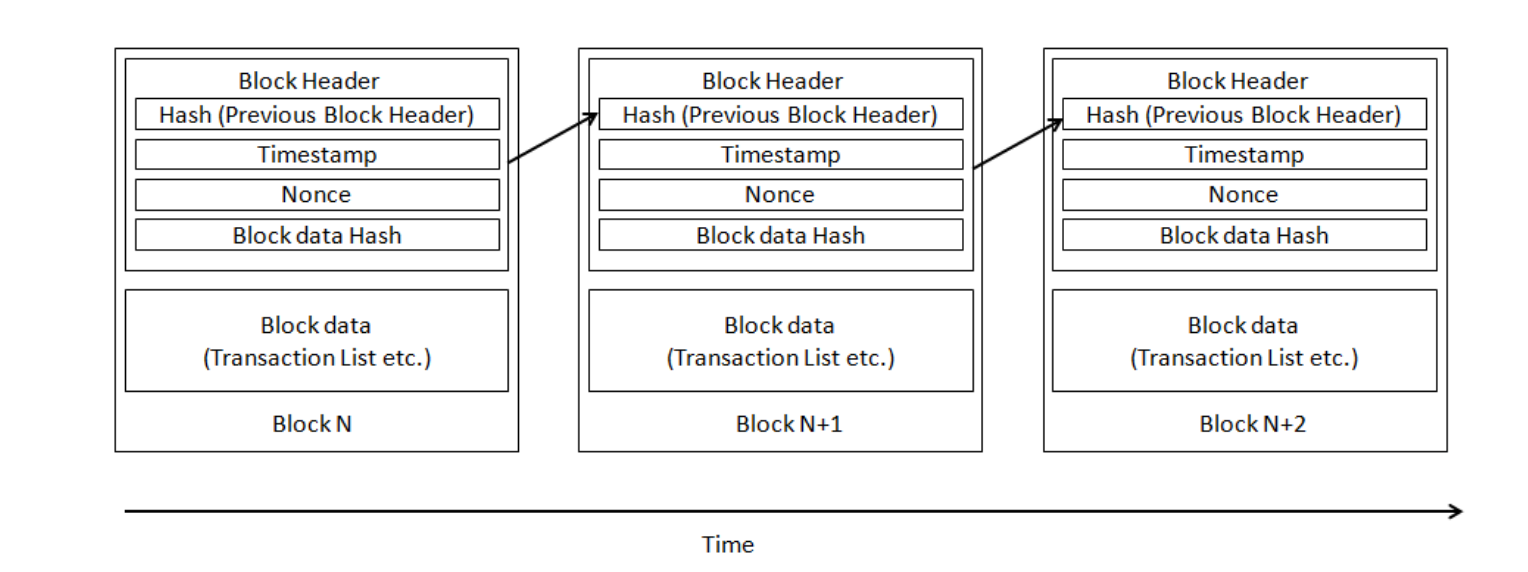
\includegraphics[width=1.95\textwidth]{images/chap01_BlockChain.png}
		\end{minipage}
		\caption[Generic chain of blocks]{Generic chain of blocks}
		
		
	\end{figure}
	
\end{center}
Blockchain has four main concepts: \\
\textit{P2P network:} nodes can interact with each other using the private and public key. Private keys are transaction signature and public keys are the address of transactions that can be reachable on the network. \\
\textit{Open distributed ledger}: It is like a book containing all transactions that each node has a copy of data and there is no central entity and anyone can see assets and how much assets has each node. Thus, they can decide about the validity of transactions.\\
\textit{Synchronization}: As all node has one copy of the ledger. Therefore, synchronization should be done throughout networks whenever a new item or one new transaction added to the network and finally consensus will need to validate these transactions.\\
\textit{Mining: }In the distributed ledger, all nodes can not receive transaction simultaneously. To add a new item in the blockchain, the consensus of all nodes are needed and it prevents every node to add a transaction into the blockchain. Miners(buyer) are who attempt to validate the transaction to add to the blockchain.\\
\subsection{Advantage Of Blockchain}
There are several distributed system based on consensus, but the one outstanding feature that makes blockchain  more prominent then the others is that:\\
Only single record stores in each participant computer. This provides transparency to the transaction.\\ 
- Storing whole records overall networks of participating computers mitigate the probability of losing infrastructure.
- One new item is confirmed and added to the blockchain, can not be altered.
- Events are stored and accessible to any participant but required public key to be reachable\cite{Sharples}.\\
- Blockchain is the sole technology that fulfills such properties:\textit{(a)trustless}: There is no need to verify involved identities in a transaction. \textit{(ii) Permissionless}: there is neither permission nor controlling for participants in the network.   \textit{(iii)censorship resistant}: Anyone can trade on blockchain and just cryptography algorithm governs the operation that entities(participants) can trust it.
this feature and above reason make the blockchain as powerful and most secure technology in commercial events over network\cite{Panarello}.


\subsection{Limitation of Blockchain}
There are some limitations and need to cope with before blockchain can be more applicable: the proof of work that generates blocks are wasteful. Although, it helps us to remain integrity in blockchain and prevent form attacks, as blockchain gets longer this problem deteriorates.\\
Also, when blockchain grows, processing speed affects adversely. Because it needs more time to verify transactions. However, blockchain relies on a consensus of the majority to ensure security in blockchain. there is a probability of being violated by this security. Requiring the consensus cause some malicious attackers can tamper the blockchain by achieving $\%51$ of consensus and introduce their version into blockchain and validate it.
To overcome these limitations, proof of stack(PoS) used over proof of work. In POS, miners are not compulsory to solve a computational puzzle. Instead, they would be selected based on their wealth or stack in the crypto token. This will decrease the probability of a $\%51$ attack and wasting the resources.

\subsection{Type of Blockchian}

\textbf{Permissionless/ public Blockchain} This blockchain allows anyone to join to network and create consensuses such as Bitcoin and Ethereum. In a permissionless blockchain, any miner can create consensus mechanisms such as proof of work, proof of stack to validate the transaction. but as this mechanism is decentralized, it has a low rate of validity function\cite{Kalra}.

\textbf{Permissioned/ Private Blockchain}: This blockchain, the only restricted participant has the right to validate the transaction. Therefore, it provides better privacy and scale-ability. Unlike permissionless blockchain, this blockchain does not have mining computation to reach the consensus because all participants are known in this network\cite{Kalra}. \\
\textbf{Wallet} contains the ether which will be used to execute transactions\cite{Egbertsen}. \\
\begin{center}
	\begin{figure}[htb!]
		
		\begin{minipage}{0.45\linewidth}
			\centering
			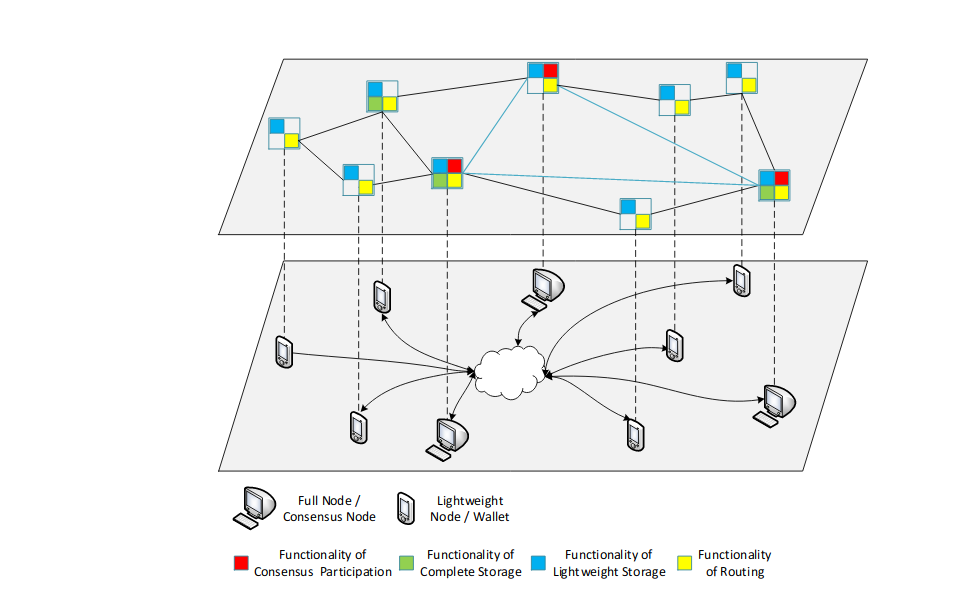
\includegraphics[width=1.85\textwidth]{images/chap01_P2P.png}
		\end{minipage}
		\caption{Permissionless blockchain network. The P2P links between consensus nodes are shown in blue.]{[60]?????}}
		
	\end{figure}
	
\end{center}

\subsection{Mining}
It is a process of computation on the blockchain to verify and add a block. Miner adds a new block and others check the validity of the new block. Any participant can take part in the mining pool, But the chance of finding valid depends on the power of the computer to perform calculations. Sometimes a miner will find an uncle block; an uncle block is a block that is initially valid but is surpassed by another, faster block. Uncle block is rewarded with $\frac{7}{8}$ of full block value and hash will be added to a valid block. A max of two uncle blocks can add to valid block and the miner of the valid block also receive $\frac{1}{32}$ extra ether for each uncle block\cite{Egbertsen}.
\subsection{Mining Pool} Mining can be done alone or in the mining pool. A mining pool is a better way to solve a block and get rewards as compared to mining alone. Miner in pool mine together and rewards will split to all members in pool\cite{Egbertsen}.
\subsection{Ether} Is the form of payment and as fuel for Ethereum. The base fo mining(find the solution and add block) successfully mining block is five ether. If the miner finds a solution but not fast, it becomes less ether like 4.375 ether and will be uncle block. Each block can contain just two uncle blocks and receive $\frac{1}{32}$ per uncle block. If another miner also finds a solution. this block can not be added into blockchain and miner just receives 2-3 ether\cite{Egbertsen}.

\subsection{Merkler Tree}
all transactions are stored in tree structure wherein leaves contain transactions and the internal node contains the hash of its subtree and a single root also contains the hash of two children and represents the top of the tree. The purpose of bottom-up hashing is that if an attacker attempts to create fake transactions into the bottom of the tree. This will change the node above and subsequently change the root. Thus altering the hash of block causing to register new block. Only the sequence of hash form root the leaf called the Merkler tree\cite{Vitalik}.   
\begin{center}
	\begin{figure}[htb!]
		
		\begin{minipage}{0.55\linewidth}
			\centering
			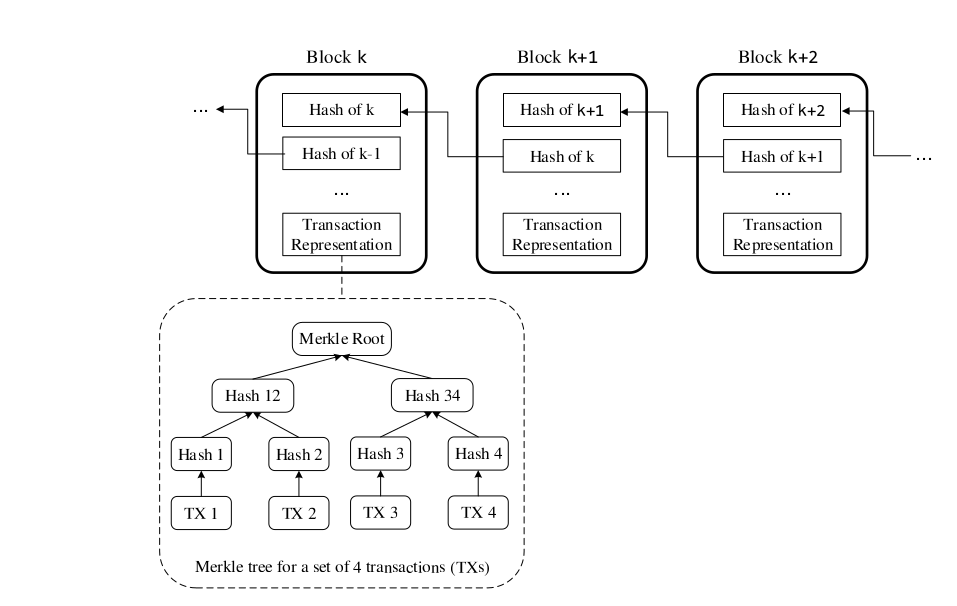
\includegraphics[width=1.85\textwidth]{images/chap01_Markler_tree.png}
		\end{minipage}
		\caption{Illustration of chain of blocks and  markler tree in single block}{[60]}
		
		
	\end{figure}
	
\end{center}
Merkler tree helps the blockcchain by providing tree-structure of transactions. The structure can be described the branches $b$ and main branch is root $b_1..._n$ and is connected by its concatenations hash $b_1.._{\frac{n}{2}}, b_{\frac{n}{2}+1}..._n$, this is:\\
\[b_1,...,_n=h(b_1,...,_{\frac{n}{2}}+ b_{\frac{n}{2}+1},...,_n) \]
And branches are :
\[ (b_1,...,_{\frac{n}{2}}, b_{\frac{n}{2}+1},...,_n)=(h(b_1,...,_{\frac{n}{4}}+ b_{\frac{n}{4}+1},...,_\frac{n}{2}) , h(b_{\frac{n}{2}+1},...,_{\frac{3n}{4}}+ b_{\frac{3n}{4}+1},...,_n))\]
Then , Binary branching continue down:
\[ b_1=h(T_1),...,b_n=h(T_n)   \]
Where T is the transaction in blockchain. Generally, it takes $\log_2(n)$ branches to check transaction is $h(T)\in b_1,...,n$\cite{Kevin}.

\subsection{Hash Function}
It is a mathematical method to apply cryptographic (secret writing) function. A hash function is deterministic means for input to produce the same output each time. Altering data generate different output. 
According to Wikipedia, the security level of the hash function has different properties: \\
\begin{itemize}
	
	\item {Pre-image resistance}: It is not easy, for initial input with $h$  hash value find the output value $m$ , in a way that $h = hash(m)$ 
	
	\item {Second pre-image resistance}: It is not easy, for input \(m_1\)  find another input \(m_2\) in way that \( hash(m_1)  = hash(m_2)\) and both have same result.
	\item {Collision Resistance} : It is difficult to find two different input \((m_1  , m_2)\) that have same output in way that\( hash(m_1) = hash(m_2)\).\\
\end{itemize}
The hash function used in blockchain and it is the most secure hashing algorithm is SHA256 which that provides the combination for a given input with 256-bit length. Using SHA256 in blockchain makes to be impossible to duplicate hash because there is a diverse combination of this input with this length and it requires a huge amount of computational works. That means there are \( 2^ {256} \) hash values\cite{Gavin}.\\

\begin{center}
	\begin{tabular}{c | c }
		
		Input value  & SHA256, message hash\\ 
		
		\hline
		1   &  6b86b273ff34fce19d6b804eff5a3f5747ada4eaa22f1d49c01e52ddb7875b4b \\
		\hline
		2    &   d4735e3a265e16eee03f59718b9b5d03019c07d8b6c51f90da3a666eec13ab35    \\
		\hline
		Blockchain & 625da44e4eaf58d61cf048d168aa6f5e492dea166d8bb54ec06c30de07db57e1 \\    
	\end{tabular}
	
\end{center}
\subsection{Blocks} Blockchain consists of blocks to record a series of transactions. Blocks are like containers that every on see metadata but only an owner has a key. Each block contains a list of transactions which once the block is accepted by the network, by some consensus algorithm, will be broadcasted to the network and included in the blockchain\cite{Egbertseng}. 

\subsection{Header} It is like metadata on the top of the block which includes a reference to the previous block, timestamp containing the time of creation, Merkle root which is an efficient data verification structure, nonce\cite{Kevin}.
\subsection{Nonce} it stands for \textit{number used only once}. It is integer number and along with block data, number, and previous hash use as input in the SHA256 function to generate the current block hash. We used this nonce to vary the hash of the current block and without modifying the data inside the block. By the usage of the nonce, a miner can generate a valid hash, adding first own block into blockchain and get the reward\cite{Gavin}.
\subsection{Merkler Root}
All transactions contained in the block can be hashed together and create a one-line hash text which is the concatenation of all transactions in the block. This is the root hash of the Merkler tree that gives a short representation of each transaction in a block????.

\subsection{Transaction} transfer data (asset) between users, an transaction contains information such:\\
- The recipients which message to send\\
- Signature of sender \\
- A mount of ether to transfer\\
- Structure value, the maximum number of computational step that transaction is allowed to do \\
- Gas price, fees that should pay…\cite{Egbertsen}.\\

\subsection{Consensus Algorithm}
The consensus algorithm is used to get the agreement of all participants about what block appends to the chain. By the use of this algorithm, real participant and malicious can be recognized. A blockchain is a consensus, if block $b_t$ is before block$b_{t+1}$  while no other participant can append block in reverse order. In this section, I will go through some important consensus algorithm which is better suited for blockchain\cite{Kevin}:
\subsubsection{Proof Of Stack}
It is an alternative to proof-of-work that fewer CPU computations for mining. In proof of stack, the chance of mining the next block 
chances of a node mining the next block depending on node balance. 
In private networks, however, where the participants are known, costly consensus mechanisms such as proof-of-work are not required. This partially removes the need for mining and give wide ranges of consensus protocol for picking node\cite{Christidis}.

\subsubsection{Proof Of Work(POW)}
It is a mechanism that ensures consensus is done without any central control. With POW miners compete to complete its transaction first into blockchain and get rewards(e.g: Bitcoin, Ether).\\
Miners connected to blockchain and accomplish task validating transactions to add new block by solving a cryptographic puzzle and anybody who complete own task sooner can add own block first in blockchain\cite{Pablo}.

\section{Bitcoin} 
The basic goal of blockchain technology is to ensure people form trustworthiness and legitimacy of transactions. Blockchain initially used to enhance commercial transactions through a currency called Bitcoin. \\
Bitcoin is the digital records or cryptocurrency that is accepted by users involved in the transaction. Bitcoin is the financial use case of this powerful technology\cite{Panarello}.
Bitcoin is the list of blocks of transactions. Each block in the blockchain is identified by the hash algorithm on the top of the block.
Bitcoin is introduced by a consensus mechanism of blockchain, it is a well-known implementation of decentralized cryptocurrency.\\
Bitcoin is the limit of the block, wherein each block is verified by a hash algorithm using SHA256 cryptography on the top of the block. Each block encompasses the hash of its parent (previous block) in the own header that refers to it.
It forms a blocklist wherein each block refers to the previous block in the list name genesis block. Altering in block implies creating a new block on the top. Since each block contains the hash of its parent creating a new block is expensive and needs proof of work that the miners allow the add new block\cite{Pablo}.
\section{Ethereum}
It is another cryptocurrency similar to Bitcoin that built on the top of the blockchain. the participant publishes the transaction on the network that is then divided into a node (called the miner) and add to the blockchain using a consensus mechanism. The state of the system refers to the sate of account that can be an external account related to the user of the system(that contains information about balance) or contract account that obtain contract code or constant storage of that account. The virtual currency in this system is \textit{Ether}. The transaction can change the state of the system by creating a new contract or invoking an existing contract. calling the external account just transfer the Ether but calling the contract account to execute the code of that contract and may perform a transaction or change the storage of that account\cite{Ilya}.

\subsection{Gas} Transaction in Etheruem platform needs fuel to execute called gas which is used internally and paid in advance to execute a transaction. If the transaction gets run off gas, means the transaction is executed. If transaction rolled back but consumed gas will not be returned.\\
To enable easier calculations, Ether also has some sub-denominations\cite{Egbertsen}:\\
\begin{itemize}
	\item Wei - $10^0$
	\item Szabo - $10^12$
	\item Finney - $10^15$
	\item Ether - $10^18$
\end{itemize}
\subsection{Account}
There are two types of accounts in Ethereum:\\
- \textit{Normally controlled} is an account controlled
by the private key. if Person has the private key can send message and ether from this account.\\
- \textit{Contract} is an account controlled by code. It is a normal account with an extra option of containing code. Ethereum blockchain starts firing transactions from an account in which this transaction is the response of receiving transactions by an account\cite{Egbertsen}.
\subsection{Message} As already said blockchain fire transaction when receiving a transaction. When an account sends a transaction means sending a message. The message contains all attributes the same as a transaction, but $gasPrice$. the only difference between message and transaction is that message is fired by contract\cite{Egbertsen}.
\subsection{Ethereumt Virtual Machine(EVM)}

It handles the state of contracts and it builds on stack-based language with some instruction like opcode. A contract is a collection of opcode statements that are executed on EVM.  EVM can be assumed as a decentralized computer which all smart contract run. It is a network of the smaller interconnected machine but sounds to be a big computer. Transactions executed smart contract on each node on the network and each node gather transactions sent from users to block to append in blockchain to collect rewards.\\
To ensure resource handling of the EVM,  every instruction the EVM executes costs gas. Operations with more computational resources cost more gas than operations with less computational resources. Therefore, using gas is beneficial due to encourages developers to write quality applications and avoiding wasteful code. When it comes to paying for gas, a transaction fee is in small amounts of Ether, and the token with which miners are rewarded for executing transactions and producing blocks\cite{Zdun}. 
\subsection{Solidity} os high-level truing complete language with Java script similar syntax. The contract is similar to classes in an object-oriented language. The contract contains the fields as persistent storage of contracts and methods to be invoked by internal and external transactions. For interacting with another contract, either need to create a new instance of this contract or make a transaction to a known contract address.\\
In particular, Solidity provides for accessing the transaction and block information like: \textit{msg:sender} or \textit{msg:value} to access the amount of \textit{wei} transferred by transaction that invoke the method. Solidity uses some fuctions to rransfer money ro another contracts suhc as \textit{call} and \textit{send}. A value trnsfer using this function to internal call transaction which implies calling contract also execute code or may fail to execute due to insufficient gas. Another contract is \textit{fallback} function that get execute via \textit{call} and \textit{send} function was preformed \cite{Ilya}.

\section{smart contract}
A smart contract in computer science is the piece of code that is designed to execute certain terms by the predefined condition. These terms are embedded and preformed on a distributed ledger. As compared to a traditional contract that includes the third party to execute terms of condition, the smart contract has low transaction fees and is more profitable without needing to the third party.\\
\textit{A smart contract is a self-executed and self-enforced agreement.}\\
Sometimes, smart contracts and DLT are remembered as the same thing, but not. They are different technologies that are complementary to each other. However, there are several platforms in DLT on which smart contracts can execute. By existing computer and capability of executing code, why have not smart contracts developed?\\
This question shows the smart contract and DLT and the relationship between each other.
A computer is capable of executing an event such as payment of contact when pre-defined conditions met. But, that would have meant that both parties require to have programmed on their computer. subsequently, the version of codes or using the program may differ that would be another issue. \\
What DLT has done, is that to bind the parties to each other by embedded code in a distributed ledger. More importantly, DLT ensures both parties have secure transactions and the contract will execute automatically. This is the exact description of smart contracts as 'self-executed' and 'self-enforced'. 
With the advent of distributed ledger, needing an efficient query of diverse data and indexing entries become more important.\\
Within the blockchain, a smart contract is actually coded inside the block and it invokes by receiving a transaction or message and send the transaction in the response of transaction that has received then it can read, write or create the contract. \\
A smart contract is an independent factor a behalf of the user to perform some operations as long to users' goals. These goals are programmed inside the contracts as code. Each contact controlled own Ether, key as long-lasting storage to follow the constant variables \cite{Egbertsen}.\\
Let us clarify more by one example:
Consider blockchain network where \textit{Bob, Alice, and Carol} are participant and there exist \textit{2 assets X and Y}. \textit{Box} uses the smart contract that defines three functions: \textit{'deposit'}: store unit of X into a contract, \textit{'trade'} send back one unit if X instead of five units of Y  and \textit{'withdraw'} to roll back all asset into the contract.
\textit{Bob} starts activating smart contract by calling the \textit{'deposit'} function and moving 3 unit of X asset into a contract and record it in the blockchain. \textit{Alice} has 12 unit of Y, and sending a transaction and 'trade' 10 unit of Y and get back 2 unit of Y and recorded into blockchain as well. \textit{Bob} signed transaction to \textit{'withdraw'} function. Contract check signature and \textit{'withdraw'} is called by owner, then transfer all deposits 1 unit of x and 10 unit of Y to Bob\cite{Christidis}.\\
There are some features of smart contact out of this example:

\textbf{-} Contract has its states and control over them. These states can be updated by executing the contract. The blockchain keeps a record of all previous states of a contract because overwriting the previous state would involve overwriting records earlier in the blockchain.\\
\textbf{-} Contract allows us to do business logic in code. \\
\textbf{-} Contract is deterministic means for the same input produce the same output.\\
\textbf{-} Smart contracts can be used to implement dynamic data storage.\\
\textbf{-} Correct smart contract describes all possible results.\\
\textbf{-} Data explains Relationship between participants.\\
\textbf{-} Smart contract is triggered by receiving a transaction and sent the transaction afterward.\\
\textbf{-} Since contract stores on the blockchain, that can be visible by every participant on the network.\\
\textbf{-} Each participant can trace contract operation due to \textit{sign} message using cryptographically verification.\\

\subsection{Security in Smart contract}
A survey on the smart contract shows that the Bitcoin and Ethereum focused mostly on financial contracts. That's why the smart contract must execute and perform correctly. 
A security issue in such a structure is to be used for a malicious purpose such as DAO hack or some incidents in Bitcoin. Such incidents 
caused a hard fork of blockchain to mitigate the malicious transaction.
Atzei et al. list 12 vulnerabilities that are assigned by Solidity, EVM, and blockchain. Such vulnerabilities can be addressed by secure smart contracts\cite{Zdun}.
\subsection{Vulnerabilities in Ethereum Smart Contracts}

Atzei et al. in this section categorized the vulnerabilities in smart contracts into three classes(solidity, Ethereum virtual machine, blockchain:\\
\begin{center}
	\begin{tabular}{c |c }
		\hline
		Level & Vulnerabilities \\
		\hline
		\multirow{2}{4em}{Solidity} & Call to the unknown \\ & Gasless send \\ & Exception disorders  \\ & Type casts \\ & Reentrancy \\ & Keeping secrets \\
		\hline 
		\multirow{2}{4em}{EVM}& Immutable bugs \\ & Ether lost in trasfer \\ & Stack size limit \\
		\hline  
		\multirow{2}{4em}{Blockchain} & Unpredictable state \\ & Generating randomness \\ & Time constraints \\
		\hline
	\end{tabular}     
	
\end{center}

\textbf{- Call to Unknown:} One invokes the function and transfer the ether to the counterpart. If there is no signature in the given address, then the callback function is executed.\\ 

\textbf{- Exception disorder: } this has occurred in a situation such as execution run out of gas, call stack limit, and \textit{throw} command.

\textbf{Gasless send: }\textbf{send} function , transfer ether to contract. This function compiled the same way of \textit{call }function without signature and returns \textit{out of gas} exception.\\
Assume \textit{call} has no signature, so it invokes \textit{callee's } fallback  function. However, the upper bound of the unit of gas is 2300 that is available to \textit{callee } and is executable.

\textbf{Type casts} compiler in solidity may be faced to some errors such as assigning an integer to type string\\
\textbf{Reentrancy} the nature of transaction cause the programmer to believe that invoking non-recursive function can not \textit{re-enter} before termination. But it is not always true, because callback function may allow the attacker to \textit{re-enter} caller function which cause the unexpected behavior or invocation loops and consume all gases.\\
\textbf{Keeping secrets} Fields of contract can be public and private. However, using a private field can not guarantee its secrecy. Because the executing contract will publish transactions on the blockchain. using suitable cryptographic techniques can remove this problem.  \\
\textbf{Immutable bugs} AS contract publishes on a blockchain, that can not be changed anymore, if there is an error on contract, it can not patch it. there is no way to predict the error of contract and terminate implementation. \\
\textbf{Ether lost in transfer} when the ether associated with any user or address.  ether will lose forever. programmer must be sure to send ether to a valid user address. \\
\textbf{Stack size limit} whenever contract call another contract \textit{call stack} increases one frame. \textit{call catack} is bounded 1204 frames: when the stack exceeds this limit size.  A further invocation will give an exception.\\
\textbf{Unpredictable state} when users send transactions on the blockchain to call smart contracts. Users can not be sure if the contract transaction time and transactions received by the user are in the same state. Because other transactions have changed the contract state. \\ 
\textbf{Generating randomness} many contracts generate random numbers where all miners chose a unique initialization seed.  \\
\textbf{Time constraints} or timestamp is used to determine which actions are mandatory in the state. \\
